\section{Additional Details and Figures}
\label{app:details}

\para{Example prompt.}
An \rte prompt with $K=2$:
\begin{lstlisting}
Decide whether the premise entails the hypothesis. Answer yes or no.

Premise: ...
Hypothesis: ...
Answer: no

Premise: ...
Hypothesis: ...
Answer: yes

Premise: <test>
Hypothesis: <test>
Answer:
\end{lstlisting}

\para{Reproducibility.}
We use seeds 42 (design), 1042 (extension sets), 7 (probe label choice) and 0 (bootstrap).
Software: vLLM 0.31, PyTorch 2.13, CUDA 13, pandas, SciPy and rouge-score.
Classification scoring uses \texttt{allowed\_token\_ids} with \texttt{logprobs\_mode=processed\_logprobs}.
Main sweeps on the shared A6000 took about 5 (0.5B), 7 (1.5B), 30 (3B), 74 (7B) and 68 (14B) minutes; probes took 5--50 minutes each.

\para{Additional sensitivity measures.}
\Figref{fig:app_sd_flip} shows the standard deviation across orders and the prediction flip rate as functions of $K$. Both behave like \pgap: roughly flat from $K=2$.

\begin{figure}[t]
\centering
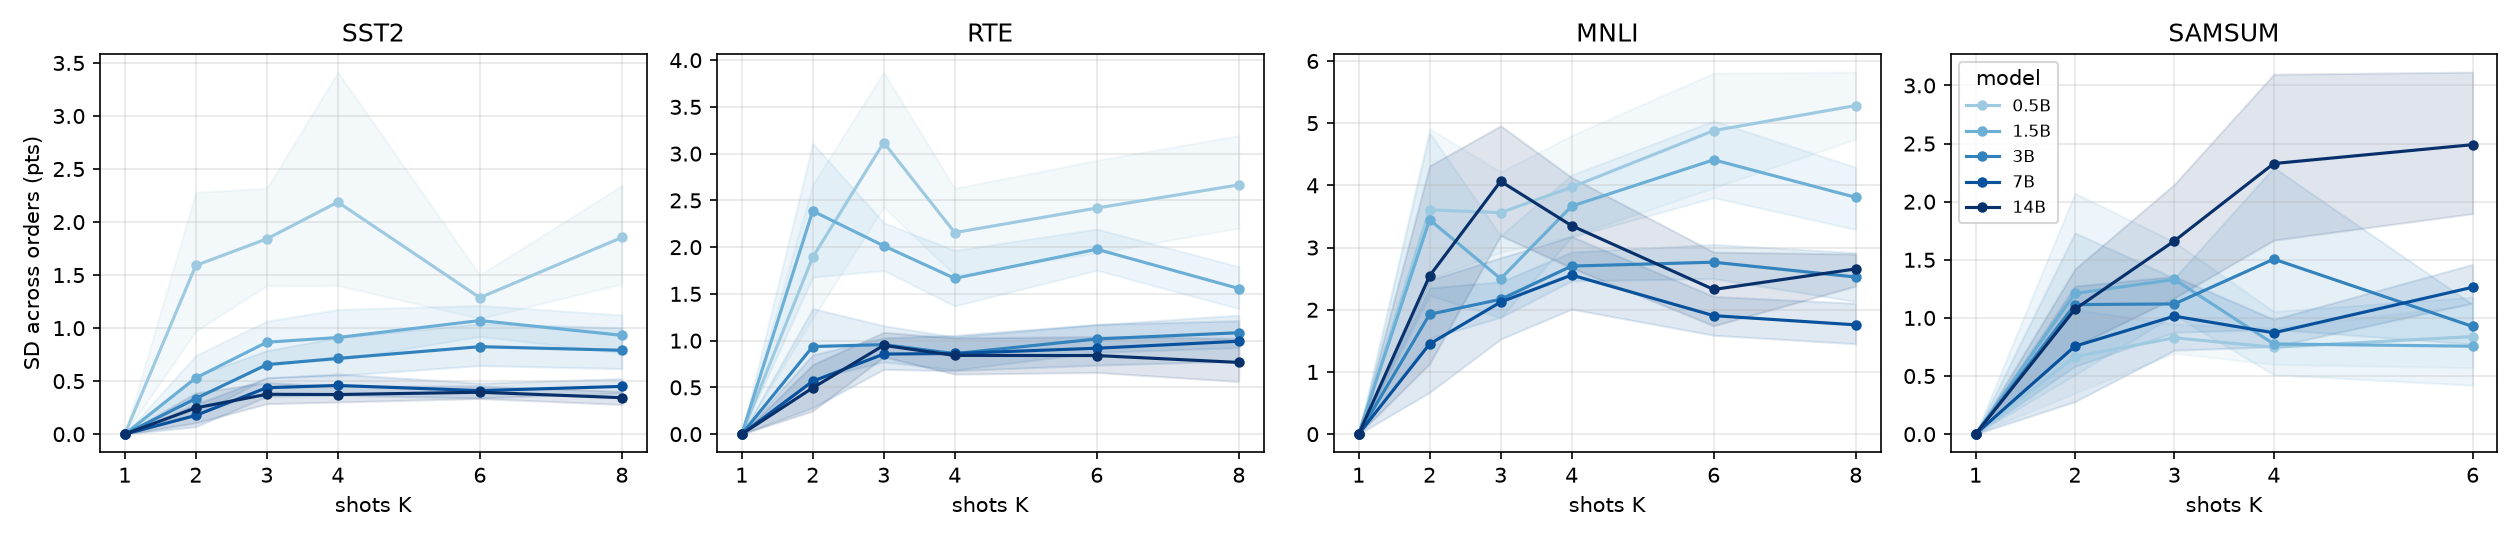
\includegraphics[width=0.95\linewidth]{figures/fig1b_sd_vs_K.png}
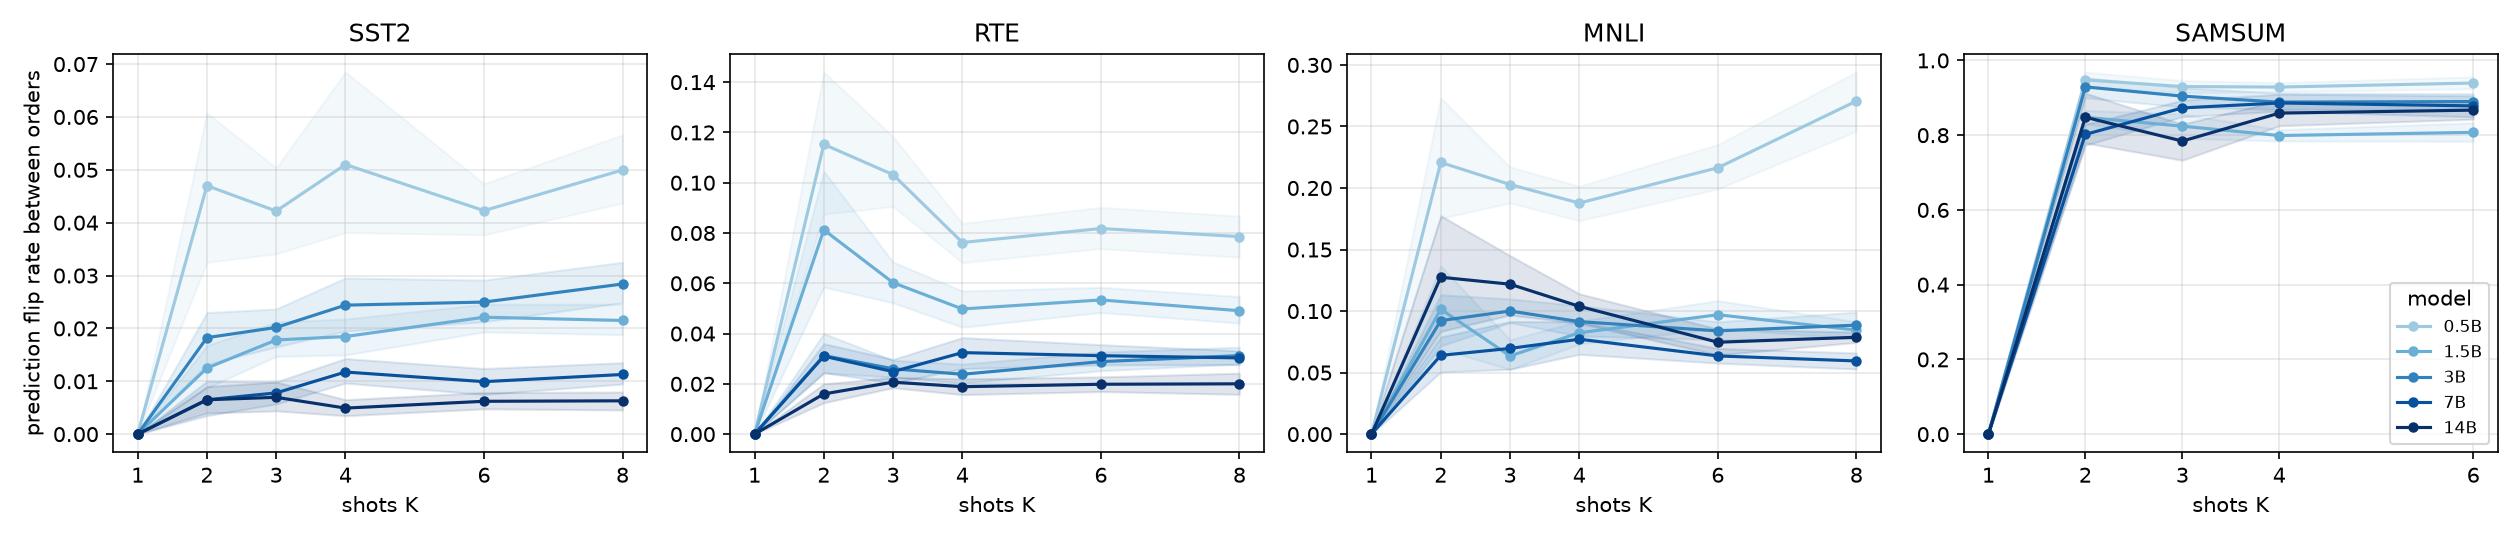
\includegraphics[width=0.95\linewidth]{figures/fig3_flip_vs_K.png}
\caption{\figtop Standard deviation of the metric across orders \vsx $K$. \figbottom Prediction flip rate between two orders \vsx $K$ (classification).}
\label{fig:app_sd_flip}
\end{figure}

\para{Accuracy by shot count.}
\Figref{fig:app_acc} plots the full accuracy curves summarized in \tabref{tab:accuracy}.

\begin{figure}[t]
\centering
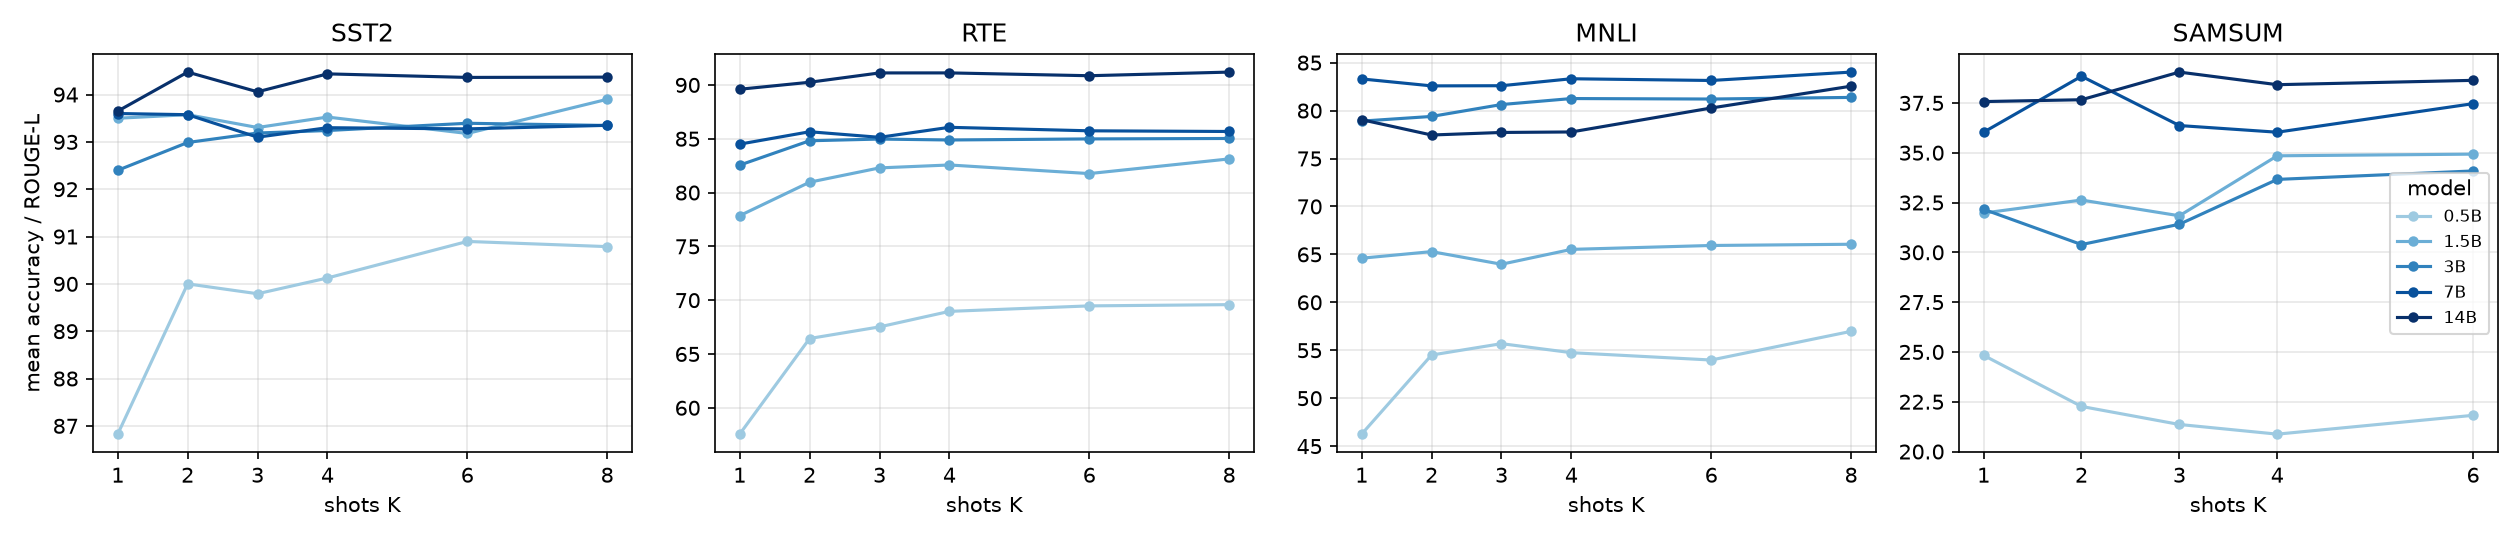
\includegraphics[width=0.95\linewidth]{figures/fig0_acc_vs_K.png}
\caption{Accuracy (\rougel for \samsum) \vsx shot count for each model.}
\label{fig:app_acc}
\end{figure}

\para{Observational position estimates.}
\Figref{fig:app_obs} shows the observational estimates: a regression of the label score on the label at each position (classification), and regressions of output length on demonstration summary length and lexical copying by position (generation). Absolute per-position values in the classification regression are poorly identified because they come mostly from label-composition differences between 10--20 demonstration sets, which are confounded with demonstration content; only within-set last-minus-first contrasts are clean. Lexical copying is under 1.5\% of output words and shows no consistent primacy.

\begin{figure}[t]
\centering
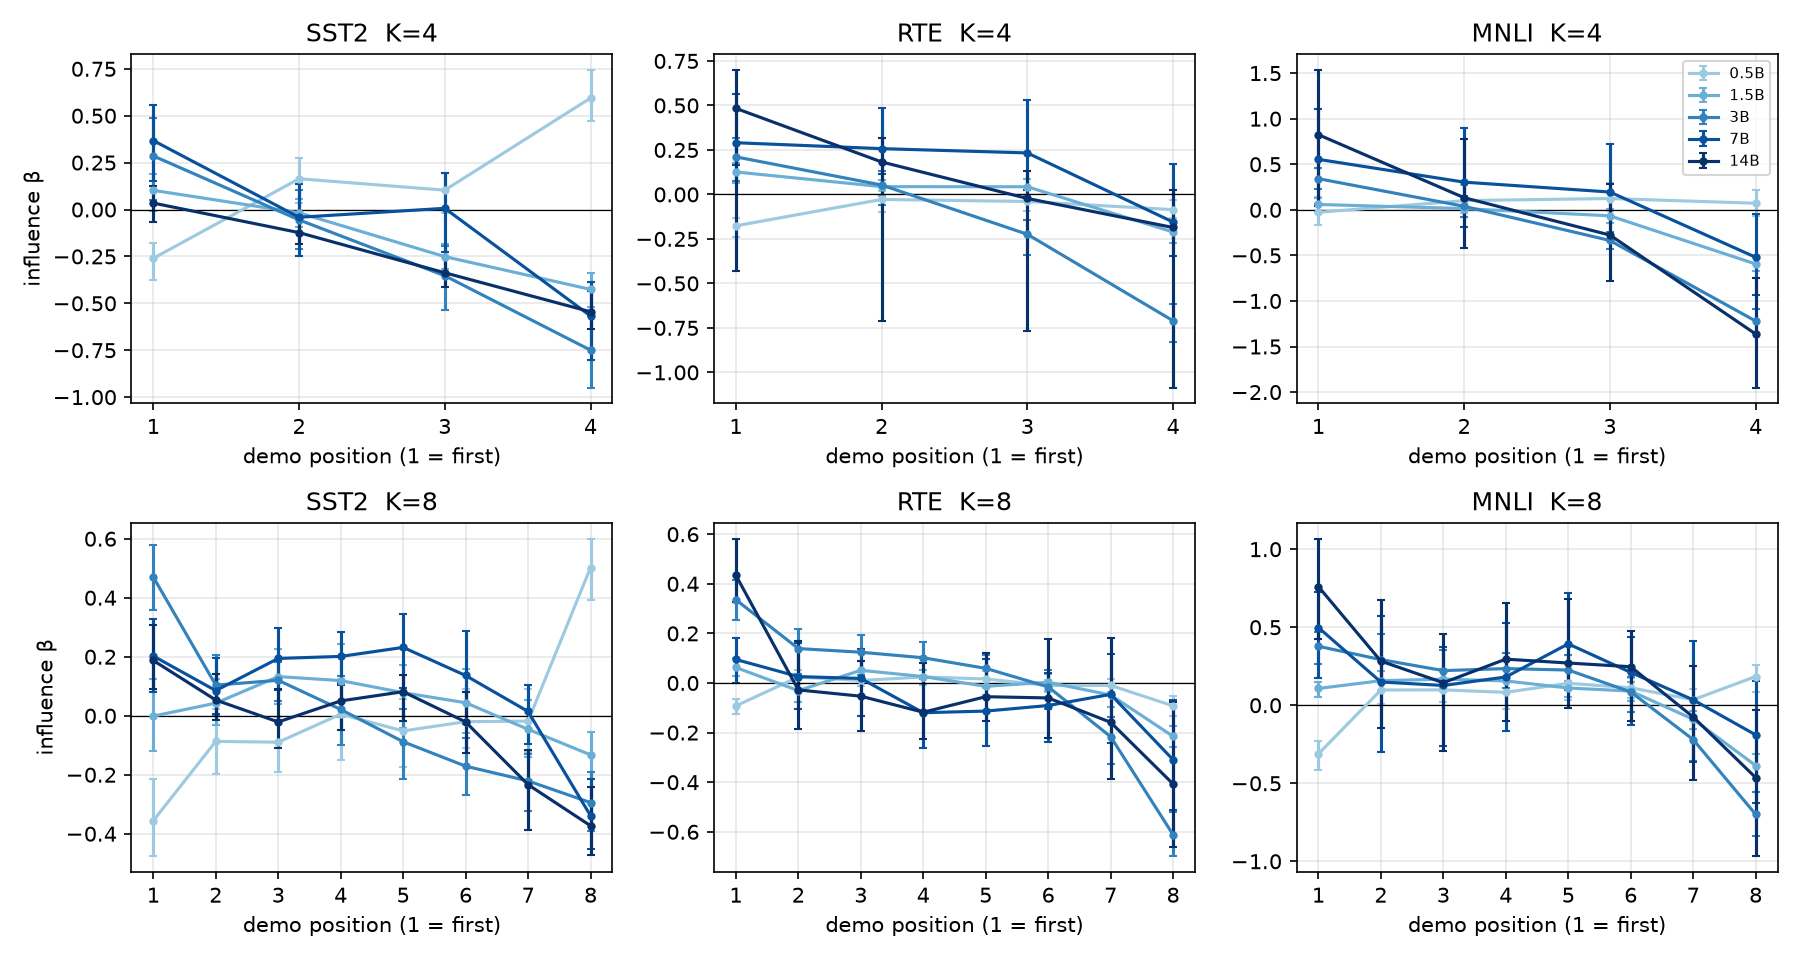
\includegraphics[width=0.95\linewidth]{figures/fig4_cls_position_influence_regression.png}
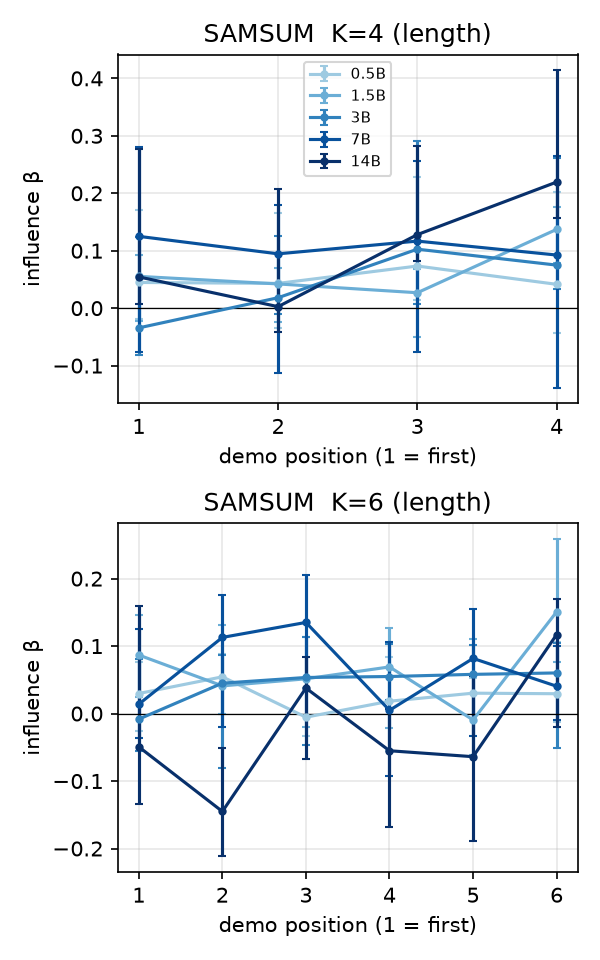
\includegraphics[width=0.4\linewidth]{figures/fig5_gen_length_influence.png}
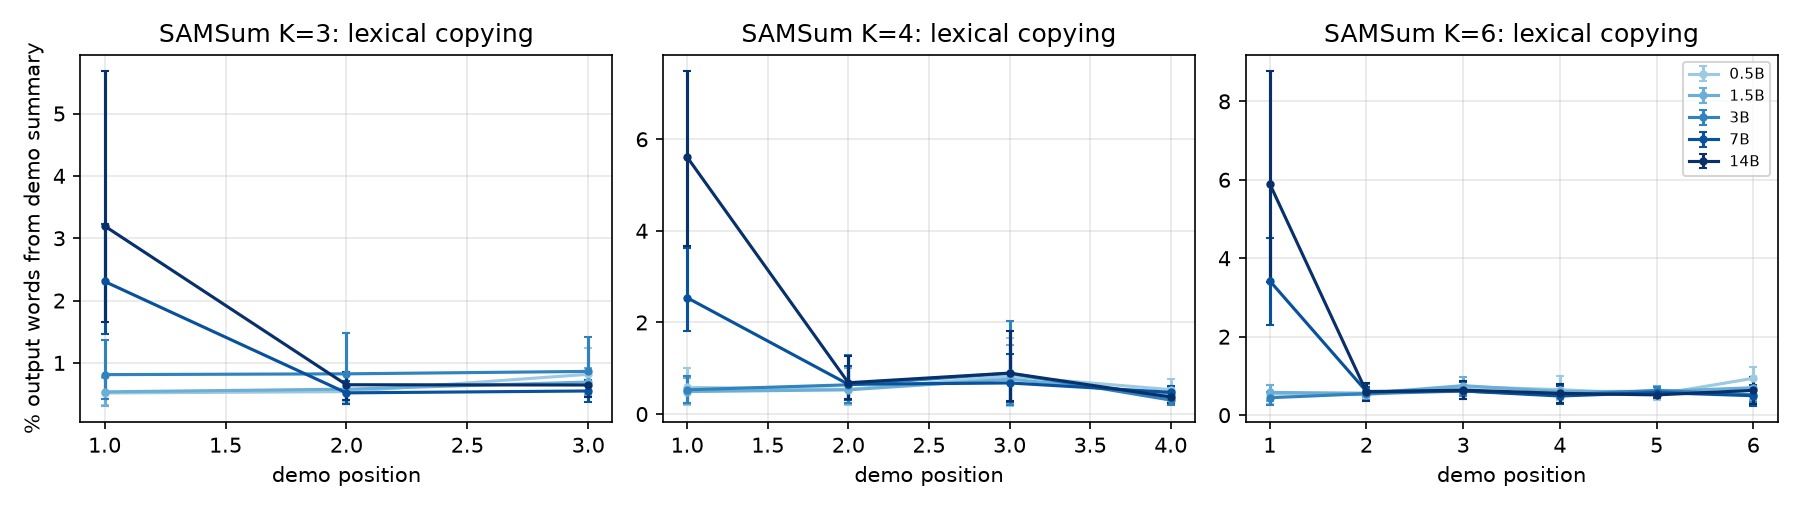
\includegraphics[width=0.95\linewidth]{figures/fig6_gen_copy_by_position.png}
\caption{Observational (non-causal) position estimates. \figtop Regression-based classification influence. Middle: regression of output length on demonstration summary length by position (\samsum). \figbottom Lexical copying of each demonstration's summary words into the output, by position (\samsum).}
\label{fig:app_obs}
\end{figure}
